\section{Camera Offsets}

After rather simple integration of the keyed video signal into the scene, where 
the 3D environment is used as background, I have observed an offset between the 
render image from the scene and the captured footage from the camera. After 
reading further into the specification of the Inogeni 4K2USB3 where it states 
that the conversion takes two intrinsic frames for encoding. The sent framerate 
of the camera is at 25 frames per second. This would mean, in theory:

\eq{offsets:timing:1}{
	t = 2 * 1 / fps
}

Assuming 30 frames per second, that is $\frac{1}{30}s$:

\eq{offsets:timing:2}{
	t = 2 * 1 / 30 \frac{1}{second}
}

\eq{offsets:timing:3}{
	t = 66ms
}

The observed offset is however far longer and is at about 260ms and therefore 
noticeable in any motion video.

\todo[inline]{There will be a sample video here.}

To mitigate this offset there are two options:

\begin{my_list}
	\item Change the camera - in example for a webcam, which usually has a 
	lower offset, ranging between 5 - 50ms. That would degrade the image 
	quality significantly but would enable perfect rendering conditions inside 
	the engine.
	\item Capture virtual images of the 3D environment and keep them on the GPU 
	until a video frame is loaded onto the GPU for usage. This keeps the image 
	quality but needs reasonable effort to reproduce the rendering conditions 
	when the video frame was taken. 
\end{my_list}

My solution uses the secondary solution, since it is able to minimize any kind 
of offset between render image and video image, the setup can stay dynamic and 
it is little to no difference to switch to a webcam-integrated solution, than 
an encoding box.

\begin{figure}[htb]
	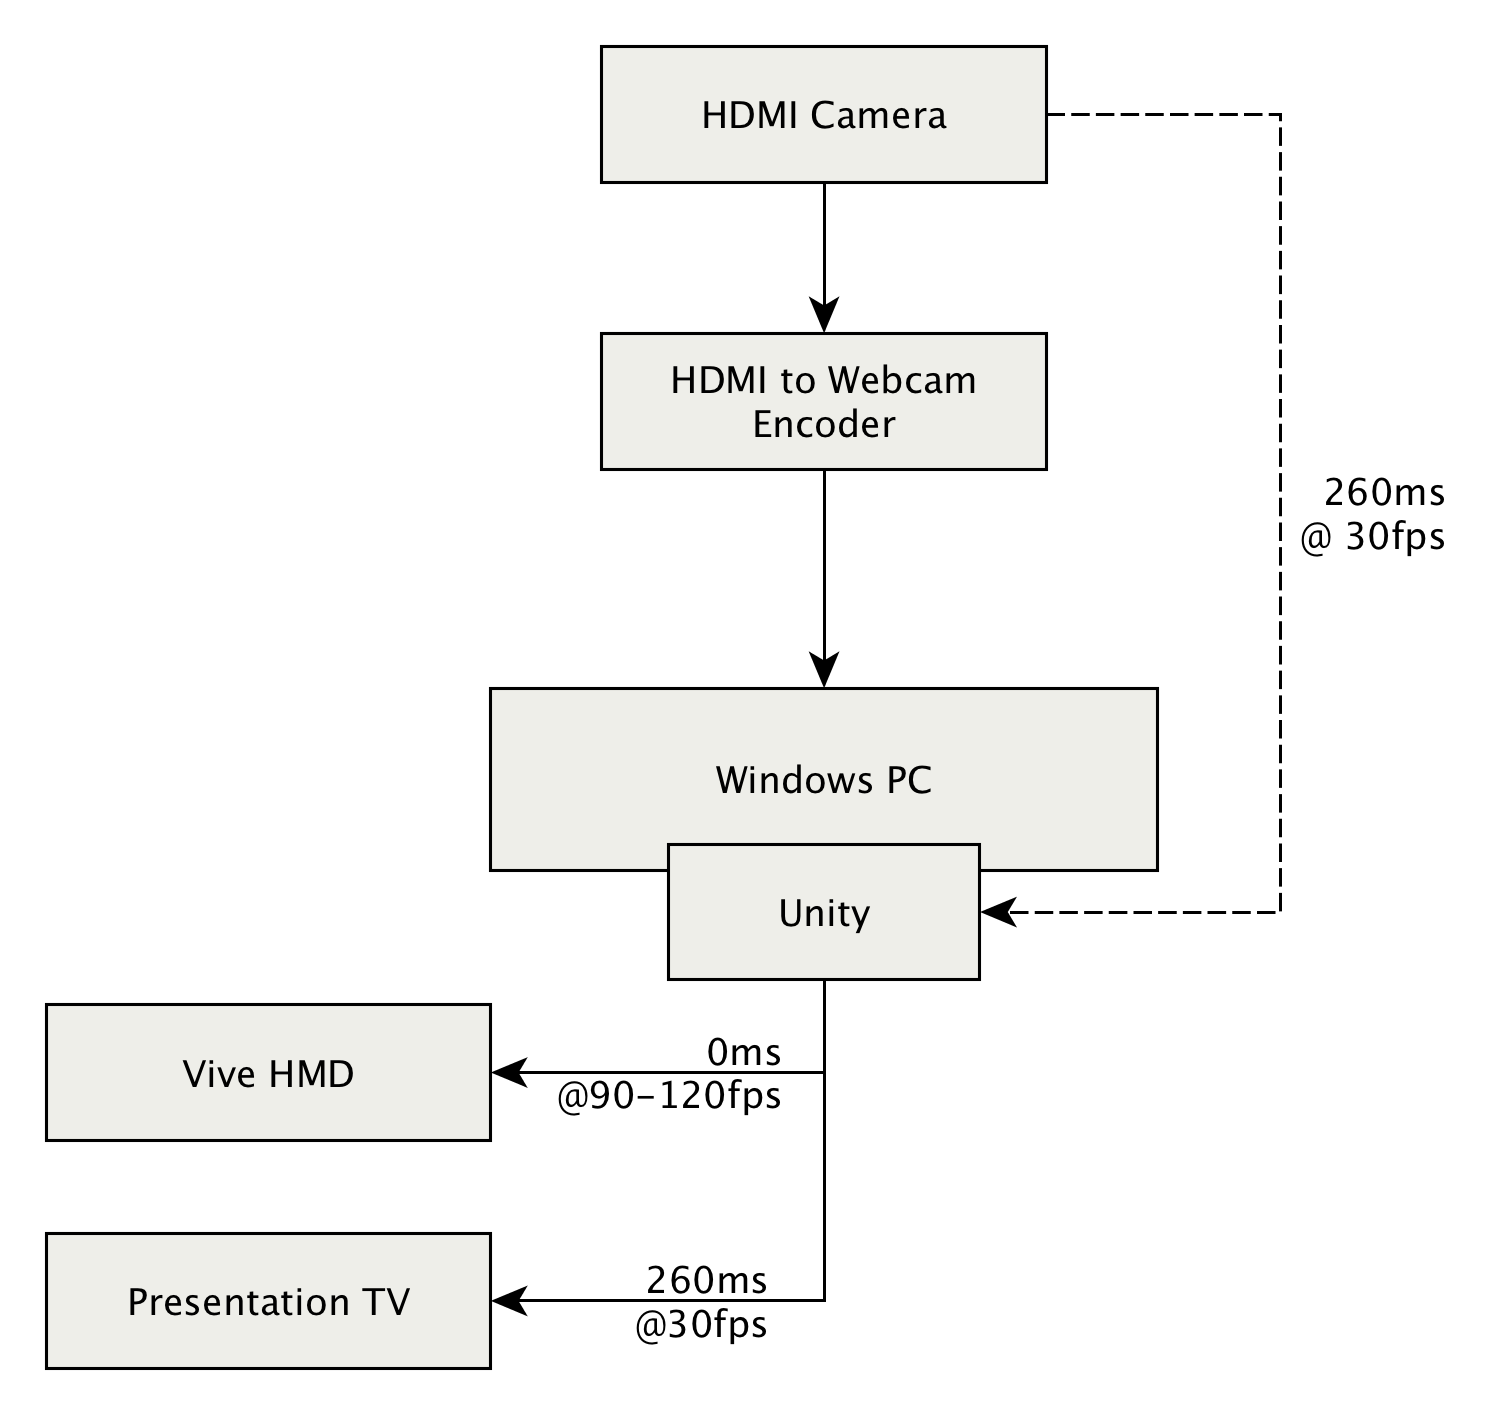
\includegraphics[width=\textwidth]{gfx/FPS-Timing-Components.png}
	\caption{Components in considering timing offsets}
	\label{fig:offsets:components}
\end{figure}

Based on the component diagram \ref{fig:offsets:components} there are two 
important notes: The time offset between camera to Unity and the TV and Vive 
HMD framerate differs. At time of writing Unity does not support dynamic 
framerates on multiple cameras. It is possible to manually initiate a render, 
however, this causes the render loop to mistime and yields to inconsistent 
frame timings inside the HMD.

\todo[inline]{kinda weak text, it's a lot of random words imo}

To conclude: The software has to store a set amount of framebuffers and cycle 
them at the right frame to guarantee minimal delays between camera and 3D 
environment.
\newline

Noteworthy is that the render loop can be 45 or 90 fps, depending on scene 
complexity, slow system performance or - in case of Unity - garbage collection, 
that could halt the engine. To account for this a strategy is needed in which 
Unity's \code{Time.deltaTime} property is used, which describes the time 
between the last and current frame.

\subsection{Framebuffer Swapper implementation}

Unity has a well engineered engine loop. It has a

As initial data needed is \code{cameraFPS}, \code{cameraOffset} and 
\code{Time.deltaTime}. From there it is possible to calculate the remaining 
data for this algorithm:

\begin{lstlisting}
	frameWindow = 1.0 / cameraFPS;
	delayCnt = cameraOffset / frameWindow;
	frameDelay = (int) delay * frameWindow;
	fractionDelay = delay % (1 * frameWindow);
	innerTimer = 0.0;
	absoluteTimer = 0.0;
	while(true) {
		innerTime += Time.deltaTime;
		absoluteTimer += Time.deltaTime;
		localTime = innerTimer - fractionDelay;
		if(localTime < frameWindow ||
		   absoluteTimer < initialDelay) {
			continue;
		}
		
		innerTimer %= frameWindow;
		absoluteTimer %= (1f + initialDelay);
	}
\end{lstlisting}

\section{Mitigating Frame Jitter}